\documentclass{article}
\usepackage[utf8]{inputenc}
\setlength{\parindent}{0pt}
\addtolength{\hoffset}{-3cm}
\addtolength{\textwidth}{6cm}
\usepackage[francais]{babel}
\usepackage{fontspec}
\usepackage{amsmath}
\usepackage{amsfonts}
\usepackage{xcolor,graphicx}

\usepackage{float}

\title{BallDroid - Android Project}
\author{Maxime Lovino}
\begin{document}
\maketitle
\begin{figure}[H]
    \centering
	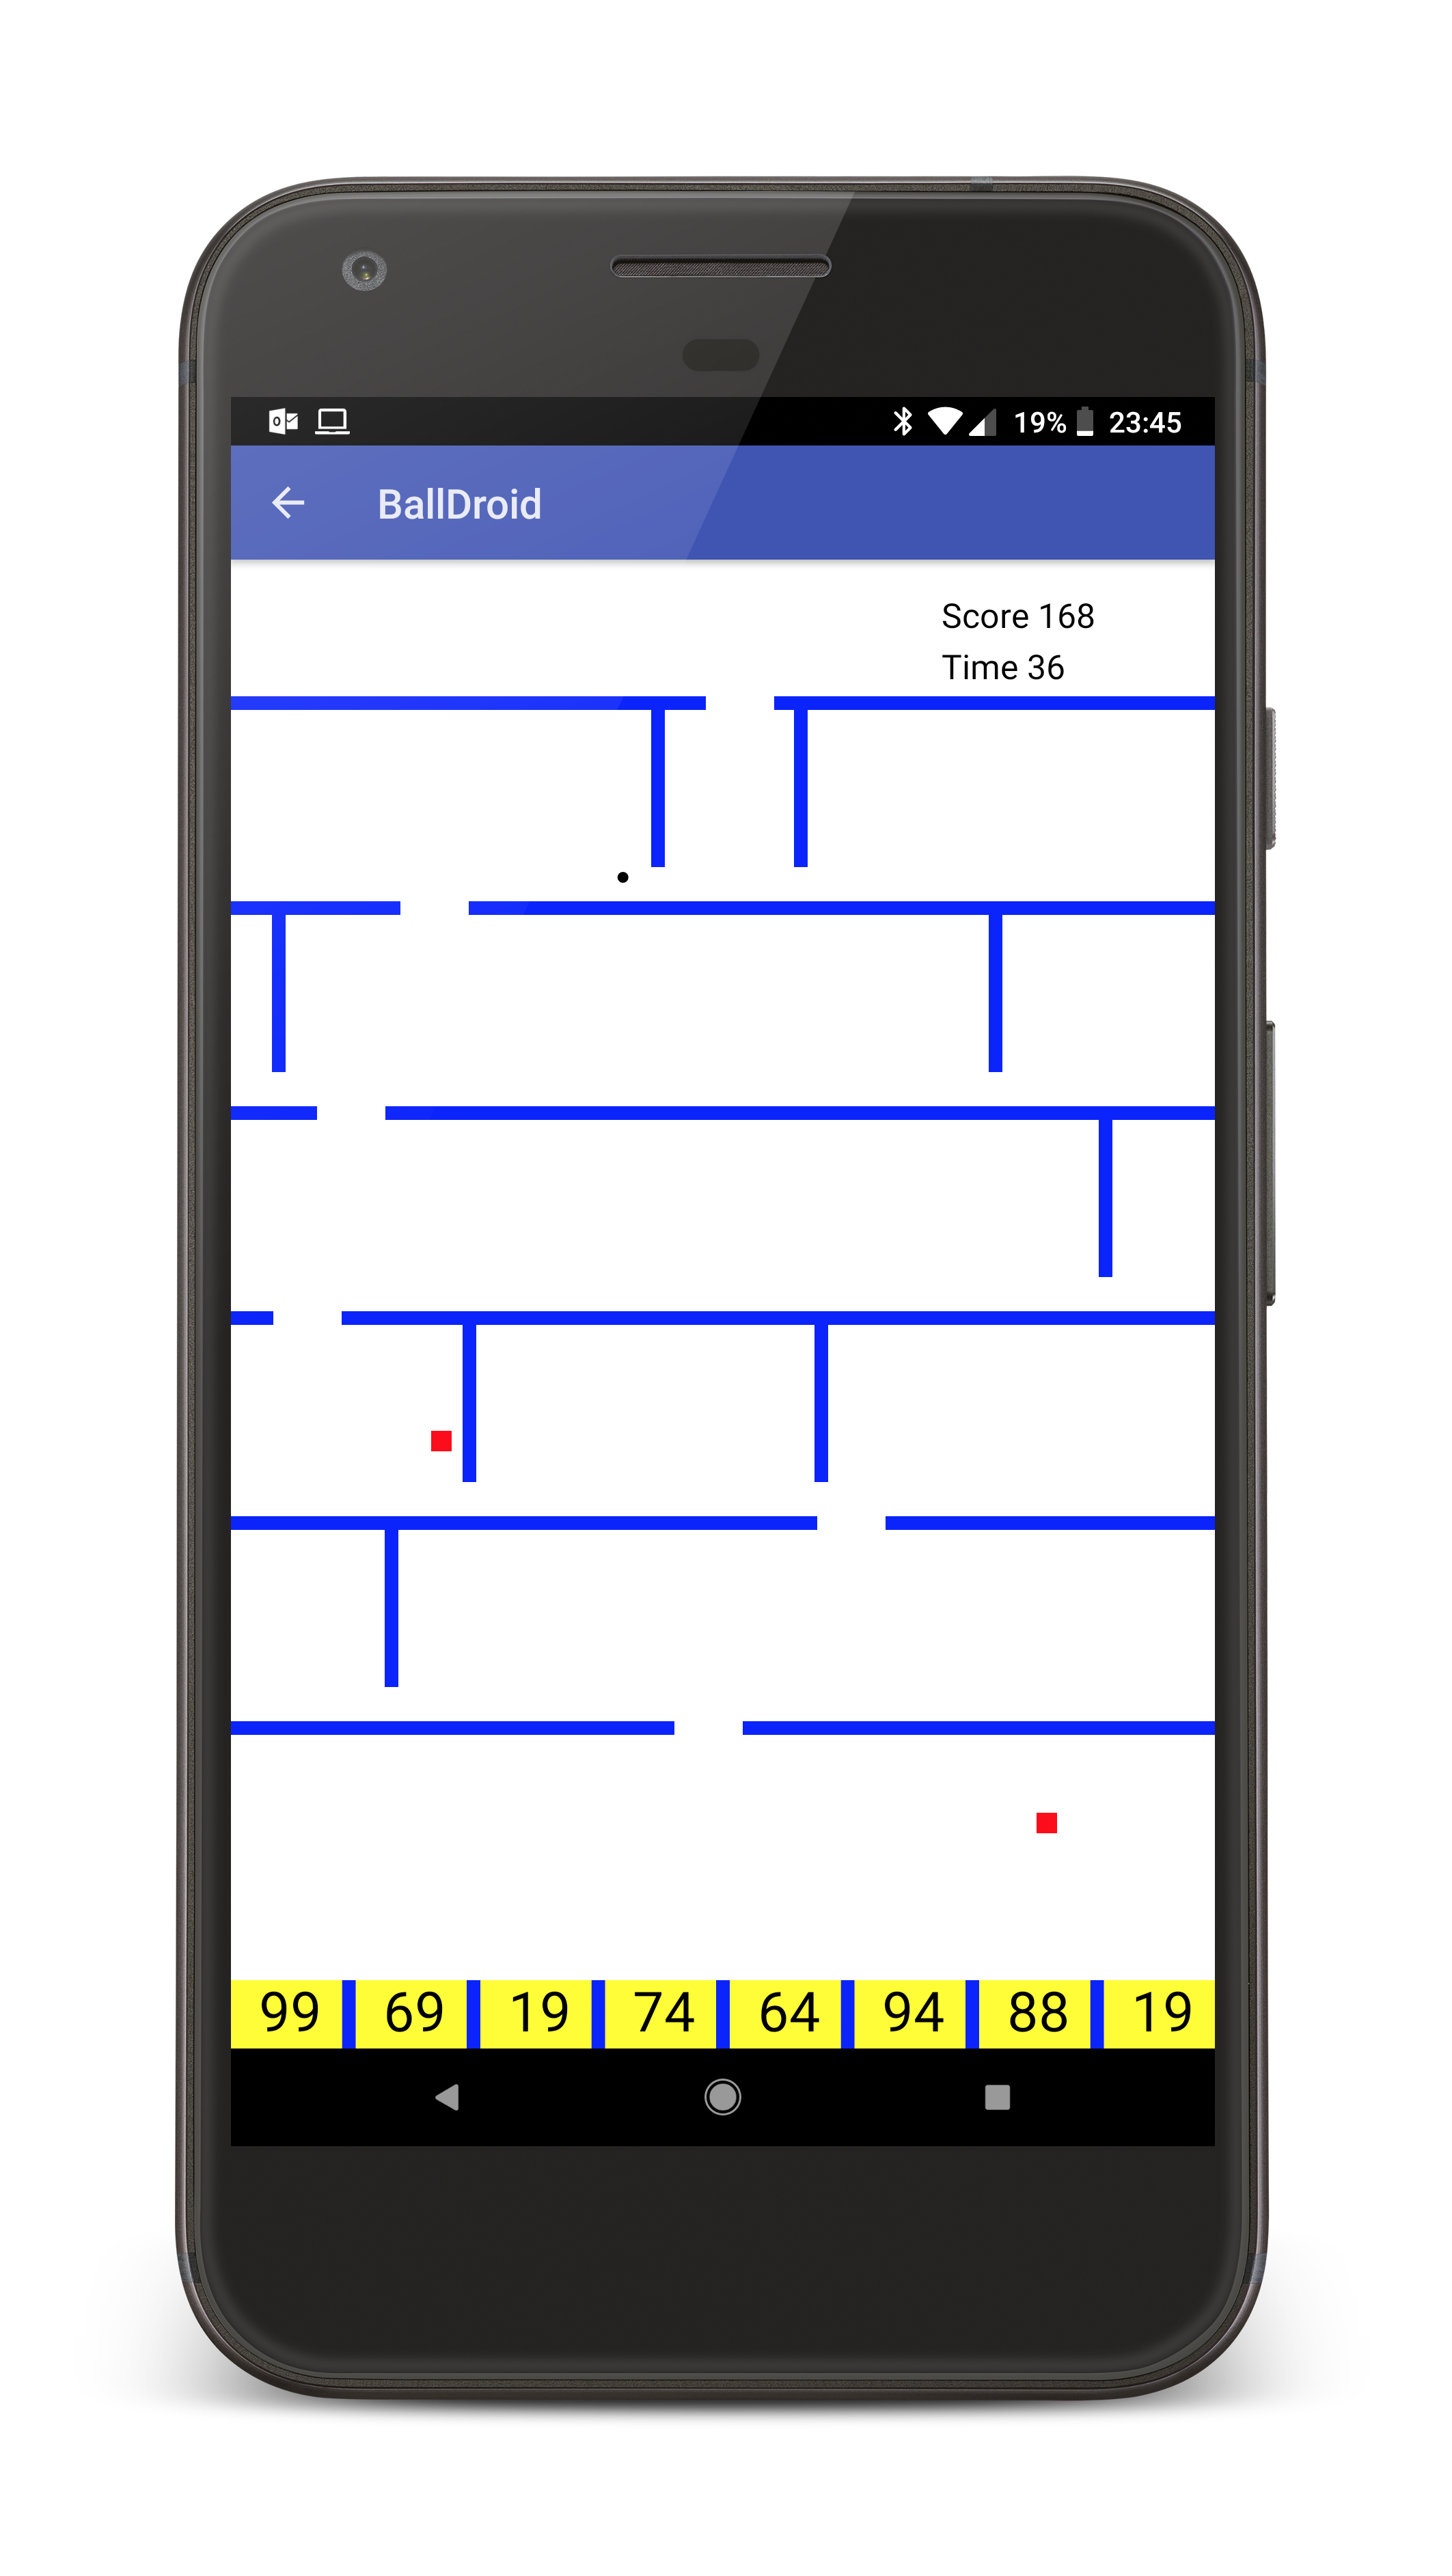
\includegraphics[height=0.7\textheight]{BallDroid_Device_Screen.png}
\end{figure}
\newpage
\section{Introduction}
BallDroid est un jeu Android tirant parti de l'accéléromètre présent dans la plupart des appareils mobiles pour diriger une balle qui tombe à travers des obstacles en vue d'arriver dans des zones définies par des points et empocher le plus de points possibles dans un temps limité. Au cours du jeu, le joueur peut récupérer des bonus et des malus qui lui permettront de gagner ou perdre du temps respectivement.
\section{Structure et spécifications de l'application}
L'application a été développée et testée principalement sur Android 8.1 (API 27) sur un Google Pixel XL avec une résolution d'écran de 2560x1440. La version minimale de SDK supportée est la version 24 (Android 7.0). L'application a également été testée via l'émulateur sur les version de 24 à 27 de l'API et des résolutions de 1920x1080 à 2880x1440.\\

L'application est composée de 4 activités: un écran d'accueil, le jeu, une vue des meilleurs scores et une page "A propos".
\section{Main Activity}
L'activité principale est assez simple et va se contenter de servir de point d'entrée au jeu, un menu a été réalisé pour choisir la difficulté, qui est définie dans l'énumération \verb+DifficultyLevel+. Au moment de lancer le jeu via le bouton sur l'écran d'accueil, la difficulté est passée dans l'Intent en tant qu'extra en passant l'ordinal de la valeur choisie dans l'enum.
\subsection{Menu}
Le menu est défini dans un fichier XML \verb+activity_main_menu.xml+ et comprend les 3 niveaux de difficultés sous la forme de Radio Buttons et une entrée pour accéder à la page "A propos". Par défaut le niveau de difficulté est le niveau le plus simple. Le niveau de difficulté choisi par l'utilisateur est stocké dans les \verb+SharedPreferences+ Android sous la forme de l'ordinal de la difficulté choisie dans l'enum pour pouvoir être persistant pour l'application installée.. 
\section{High Score Activity}
L'activité High Score affiche tous les scores enregistrés dans le jeu dans l'ordre décroissant avec leur niveau de difficulté dans une \verb+ListView+ en utilisant un \verb+ArrayAdapter+ à partir d'un \verb+ArrayList+ contenant les scores. Le layout \verb+score_list_item.xml+ définit une entrée de la liste.
\subsection{Stockage des high scores}
 Le stockage de ces scores est réalisé par une base de données SQLite dans l'application (pratique commune pour les applications Android).\\
 La structure de la base de données est de sa table est définie dans le package \verb+ch.hepia.lovino.balldroid.models.db+. Il s'agit d'une table contenant un index auto-généré, le score et le niveau de difficulté. Au moment de l'affichage de l'activité High Score, un SELECT est réalisé dans la base de données en triant par score descendant.
\section{Game Activity - Le jeu}
L'activité principale de l'application est l'activité contenant le jeu, celle-ci est entièrement vide de base en terme de layout et est entièrement générée au runtime. En terme de structure, j'ai décidé d'utiliser un modèle MVC bien que pas 100\% strict par rapport à la définition MVC comme on pourra le voir. Etant donné que les modèles contiennent un petit peu de logique et de rendu pour simplifier les choses et éviter d'écrire 3 fois les classes pour rien, étant donné l'ampleur réduite du projet.
\subsection{Structures de données - Model}
\begin{figure}[H]
    \centering
	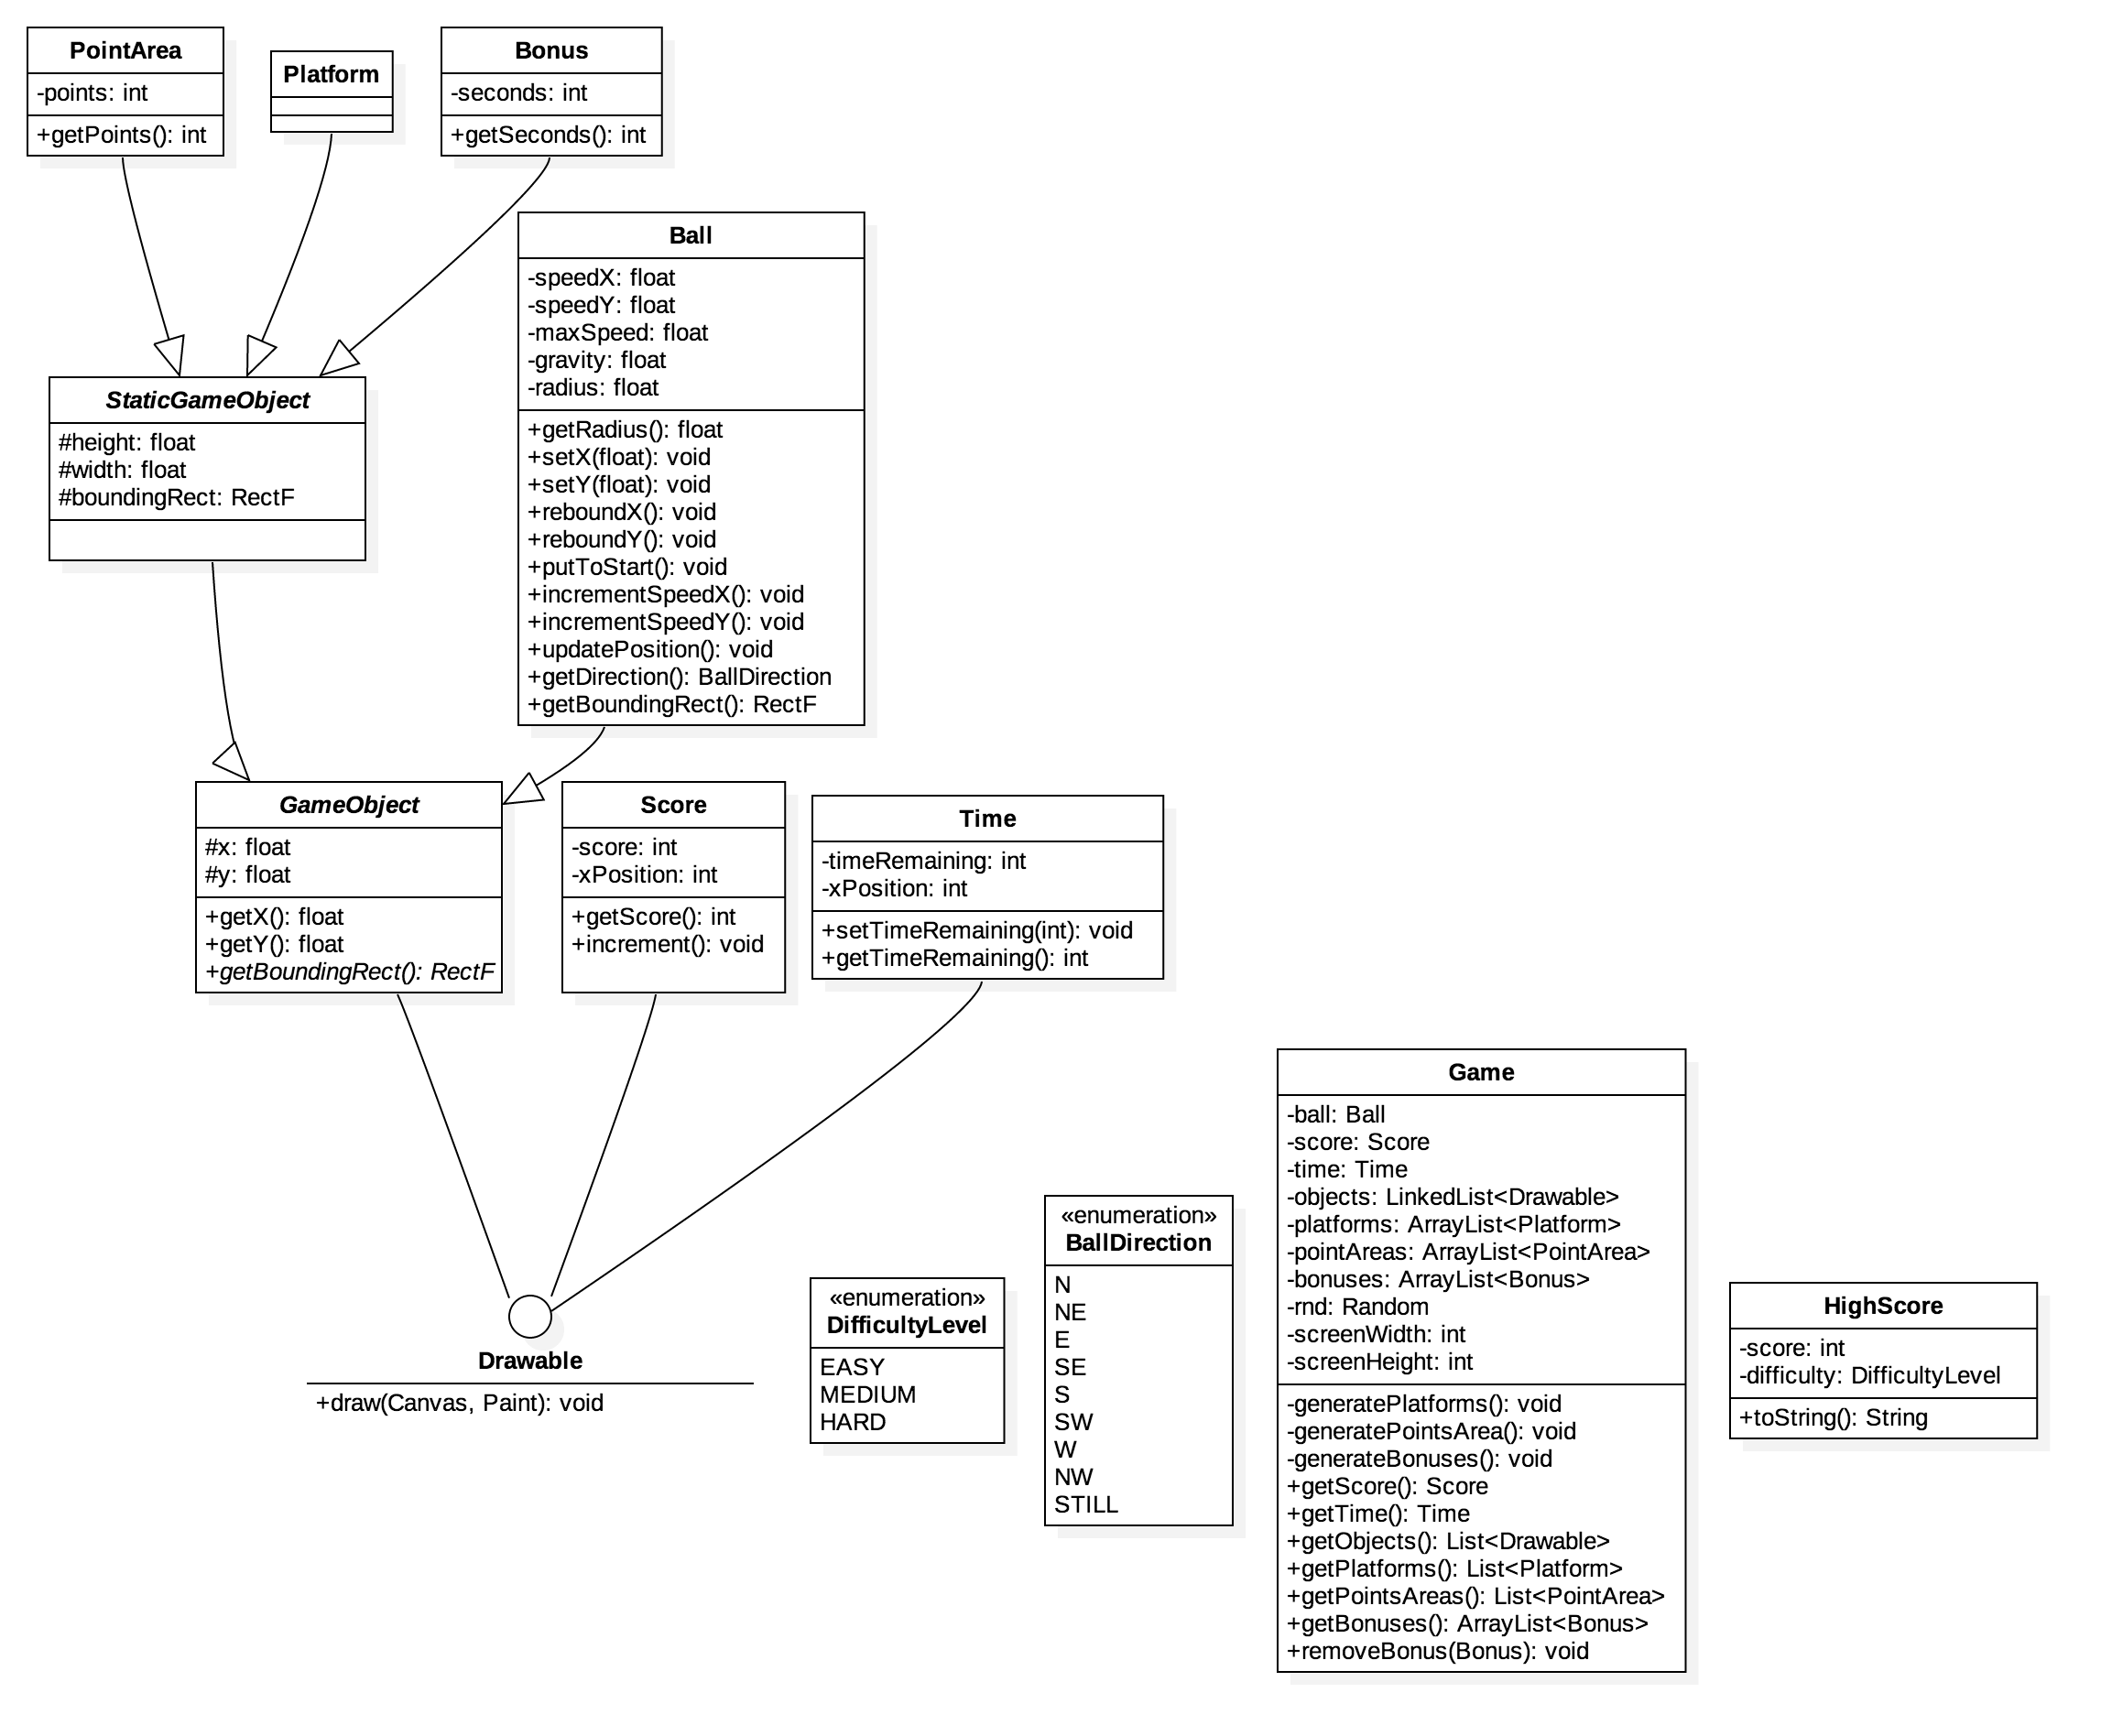
\includegraphics[width=\textwidth]{BallDroid_UML.png}
\end{figure}
En terme de modèles, j'ai réalisé une architecture tirant avantage de la POO et de l'héritage pour regrouper et catégoriser les différents éléments nécessaires pour le jeu.
\subsubsection{L'interface Drawable}
Ici est contenu en fait la plus grande digression par rapport au modèle MVC, l'interface \verb+Drawable+ qui définit une fonction \verb+draw(Canvas,Paint)+ et qui est implémentée par tous les modèles qui seront affichés à l'écran. Cela permet comme on le verra plus tard de passer à la vue une liste de \verb+Drawable+ et on pourra simplement appeler \verb+draw+ sur tous ces éléments. Si nous voulions coller au plus proche du MVC, il aurait fallu réaliser une classe de rendu pour chaque modèle et implémenter cette interface sur ceux-ci, mais cela était plus pratique de cette façon dans ce cas.
\subsubsection{Score et Time}
Score et Time sont deux classes qui définissent les deux textes en haut de l'écran affichant le score et le temps restant, ils implémentent l'interface \verb+Drawable+
\subsubsection{GameObject}
A partir de là, \verb+GameObject+ est une classe abstraite qui définit une position (x,y) pour un élément de jeu. On définit également une méthode abstraite pour récupérer la bounding box rectangle autour de l'élément qui sera définie par les sous classes.
\subsubsection{Ball}
La balle hérite de \verb+GameObject+ et y ajoute un rayon, ainsi qu'une vitesse sur chaque axe, sa force de gravité, sa vitesse maximale (ces deux dernières dépendent de la difficulté) et des constantes pour les forces de frottement et les positions de départ. Ensuite, on définit des méthodes permettant de déplacer la balle, augmenter sa vitesse, la faire rebondir (inverser sa vitesse en la diminuant) et récupérer sa direction sous la forme d'une énumération BallDirection qui est définie comme les 8 directions cardinales ou la balle à l'arrêt. Cela va nous servir pour la gestion des collisions. On implémente également la méthode pour créer un rectangle autour de la balle et le retourner pour gérer ses collisions.
\subsubsection{StaticGameObject}
La balle étant le seul élément du jeu qui bouge, j'ai créé une classe abstraite \verb+StaticGameObject+ qui hérite de \verb+GameObject+ pour définir un élément fixe, tous ces éléments sont définis comme des rectangles, donc cette classe ajoute des champs de largeur et hauteur à la classe de base, ainsi qu'une implémentation de la méthode pour récupérer la bounding box, qui sera la même pour toutes les sous-classes étant donné que tout sera un rectangle désormais.
\subsubsection{Platform}
Je n'ai pas distingué la plateforme et le mur dans mon jeu, les deux sont définis comme des plateformes, leur taille et leur position sert à les distinguer, et au niveau de leur physique ils sont gérés de la même façon de toute façon.
\subsubsection{Bonus}
Un bonus contient un certain nombre de secondes (positif ou négatif) à ajouter au temps restant du jeu, la seule différence entre un bonus est sa couleur verte ou rouge en fonction des secondes positives ou négatives.
\subsubsection{PointArea}
PointArea définit une zone d'arrivée, elle est définie par un nombre de points qu'elle rapporte au joueur.
\subsubsection{Game}
Game est en fait le modèle principal qui est appelé par le moteur de jeu. Le plateau de jeu, ses plateformes, ses bonus et ses zones d'arrivée sont générés aléatoirement dans cette classe lors de la création d'une instance de Game. Le plateau s'adapte à la résolution par exemple en définissant plus "d'étages" de plateformes si la résolution verticale est plus élevée.\\

Tous les éléments du plateau sont placés dans deux listes à chaque fois, une liste contenant tous les éléments \verb+Drawable+ du jeu (récupérée par la vue) et une liste contenant tous les éléments de leur type (une pour les bonus, une pour les plateformes, une pour les zones d'arrivées) qui seront récupérées par le moteur de jeu pour vérifier les collisions et la victoire de points.
\subsection{Le rendu - View}
Je ne vais pas m'attarder plus en profondeur sur la partie vue, car elle suit ce qui était expliqué dans le PDF fourni, on a donc une \verb+GameSurfaceView+ avec un thread d'affichage \verb+DrawingThread+ qui à chaque frame prend un lock sur le canvas et appelle \verb+onDraw+. Dans cette méthode, on appelle la méthode pour que le moteur effectue les mouvements et ensuite on récupère les éléments \verb+Drawable+ à afficher et on appelle \verb+Draw()+ sur ceux-ci.
\subsection{Le moteur de jeu - Controller}
Le moteur de jeu est la partie qui va récupérer les valeurs de l'accéléromètre (seulement sur l'axe X) et appliquer les mouvements à la balle à chaque frame, elle va aussi appeler la création du jeu, lancer et mettre en pause le timer lorsque le jeu se met en pause et gérer les collisions et les points.
\subsubsection{La fonction update}
La fonction \verb+update+ est la fonction principale du moteur de jeu. Dans cette fonction, on va, si le jeu n'est pas en pause, augmenter la vitesse de la balle en fonction de l'accélération de l'accéléromètre sur l'axe X et de la gravité sur l'axe Y et ensuite mettre à jour sa position d'une unité par rapport à sa vitesse en appelant les fonctions correspondantes dans le modèle.
\subsubsection{Les collisions en fonction de la direction de la balle}
A partir de là, nous devons gérer les collisions de la balle, tout d'abord avec les bords de l'écran à gauche et à droite, en replaçant la balle au bord de l'écran et en inversant sa vitesse. \\

Ensuite il y a la gestion des collisions avec les plateformes. Pour cela, je prends la direction de la balle, et ensuite on parcourt toutes les plateformes et on utilise la fonction \verb+intersect+ pour vérifier s'il y a une intersection avec la plateforme. Ensuite, en fonction de la direction de la balle, en cas d'intersection, il faudra faire rebondir la balle que dans certaines directions. C'est-à-dire que par exemple, une balle avec direction NE ne peut rebondir que sur le bas et la gauche d'une plateforme, même si elle pourrait satisfaire la condition de rebond sur le haut par rapport à sa position, mais cela n'aurait pas de sens compte tenu de sa direction. Cela permet donc de gérer d'une meilleure façon les collisions avec les bords et les coins des plateformes dans ce cas, car on ne fait que des rebonds logiques du point de vue physique.
\subsubsection{Zones d'arrivée}
Ensuite, on parcourt toutes les zones d'arrivée et en cas d'intersection avec une zone d'arrivée, on augmente le score par rapport aux points de celle-ci et on replace la balle à la position de départ.
\subsubsection{Prise de bonus}
Pour les bonus, on parcourt tous les bonus et en cas d'intersection, on applique le temps gagné ou perdu au temps restant et on met le bonus dans la liste \verb+bonusesToRemove+, à la prochaine frame, le bonus sera enlevé de la partie. Cela nous évite de faire disparaître un bonus avant même de le toucher, ce qui provoque un petit glitch graphiquement. A noter, l'utilisation d'une petite touche de programmation fonctionnelle en Java 8 pour le traitement de tous les bonus à enlever en utilisant:
\begin{verbatim}
this.bonusesToRemove.forEach(game::removeBonus);
\end{verbatim}
\subsubsection{La gestion des pauses}
La pause est géré dans l'activité de jeu, sur pression du bouton Back. L'activité intercepte cette pression et appelle \verb+pauseGame()+ sur le jeu qui va arrêter de récupérer les données de l'accéléromètre, arrêter le timer et mettre en pause les mouvements via un booléen. Ensuite, à la pression suivante de la touche Back, on va remettre en fonction le listener, relancer le timer avec la valeur restante du temps et débloquer les mouvements.
\subsubsection{Timer thread et fin de jeu}
Le timer est géré par un thread de timer qui est géré par le moteur de jeu. Lors que le timer arrive au bout, on utilise un Handler pour lancer la fonction \verb+endGame+ sur le thread principal (aussi appelé UIThread) qui va join le thread Timer, arrêter le jeu, enregistrer le score et notifier l'activité qui va afficher un AlertDialog avec le score de l'utilisateur et des options pour retourner à la page d'accueil ou à la vue des high scores. A noter qu'après avoir lancé une de ces deux activités, il est très important d'appeler \verb+finish()+ après le \verb+startActivity(...)+ depuis l'activité de jeu pour détruire celle-ci, autrement on pourrait retourner au jeu en appuyant sur la touche Back.
\section{Conclusion et remarques}
En conclusion, ce jeu m'a permis de me familiariser de plus en plus avec le développement sur Android et principalement avec les \verb+SurfaceView+ que je n'avais jamais utilisé auparavant. Je trouve par contre que le cours que nous avons eu jusqu'à maintenant n'était pas vraiment suffisant pour réaliser le TP, surtout du point de vue de la structure du TP et des interactions. Le gap entre les exercices et ce TP était un peu trop conséquent, du coup une grande partie de l'apprentissage nécessaire pour ce TP a été fait durant la réalisation de celui-ci. A noter que je touche au développement Android depuis déjà deux ans (pas de jeux) ainsi que pour mon projet de semestre et que donc j'avais déjà pas mal de bases, mais cela ne m'a pas empêché de devoir m'informer et apprendre avec les documentations etc.
\end{document}
